\documentclass[a4paper,10pt]{article}

\usepackage[utf8]{inputenc}
\usepackage[english]{babel}
\usepackage[T1]{fontenc}
\usepackage{mathpazo}

\usepackage[colorlinks=true]{hyperref}
\hypersetup{urlcolor=black,linkcolor=black}

\usepackage{enumerate}

\usepackage{fullpage}
\setlength{\parindent}{0pt}
\setlength{\parskip}{\medskipamount}

\usepackage{amsmath}
\usepackage{amssymb}
\usepackage{mathrsfs}
\usepackage{amsthm}
\usepackage{array}
\usepackage{graphicx}
\usepackage{comment}


\title{Project proposal}
\author{PPP \--- ENS Lyon}
\date{M1. 2014}

\begin{document}
\maketitle

\newlength{\title}
\settowidth{\title}{Coordinator }

\newlength{\object}
\setlength{\object}{\textwidth} \addtolength{\object}{-\title} \addtolength{\object}{-6.8pt} 
	\addtolength{\object}{-2\tabcolsep}

\renewcommand{\arraystretch}{1.5}

\begin{center}
\begin{tabular}{@{}|p{\title}p{\object}@{}|}
\hline
Title & Projet Pensées Profondes (PPP)\\
Coordinator & Marc \textsc{Chevalier}\\
Members & Raphaël \textsc{Charrondière}, Marc \textsc{Chevalier}, Quentin 
      \textsc{Cormier}, Tom \textsc{Cornebize}, \linebreak Yassine \textsc{Hamoudi}, 
      Valentin \textsc{Lorentz} and Thomas \textsc{Pellissier} \textsc{Tanon}.\\
Abstract & \emph{Projet Pensées Profondes} aim is to build a project about natural language question answering framework.
It would be done at the ENS Lyon, from September to December 2014, by a team of seven M1 students. This proposal presents
our subject and exposes our goals.\\
\hline
\end{tabular}
\end{center}

\section{Introduction}

\emph{What is the birth date of the first president of the United States?} This is the typical question that we would like to
answer quickly and succinctly with an automatic question answering system. This requires three steps.

\begin{itemize}
\item[\textbf{Understanding}] the natural language. The input string given in standard 
English has to be transformed into a normal form. 

\item[\textbf{Querying}] some database (e.g. Wikidata), using the normal form.
Some operations may then be applied, like performing a sort.

\item[\textbf{Displaying}] the answer in a convenient fashion.
\end{itemize}

\section{Expected results}
The first goal of the PPP is to provide a free, modular and well documented
query answering tool that will interest research communities for extensibility features. 

We expect to have in December a framework that would allow people to ask
questions in plain text through a web user interface, a core module able to transform
this question into a normal form and a demo backend module able to answer
to historical questions using Wikidata data.

We expect also to have done some research on natural languages analysis using
neuronal networks. These researches may lead, if successful, to
a small scientific article.

\section{Targeted users}

Our main purpose is to allow people to design their own modules and
easily include them in the tool. For example, sports modules could be done to 
answer questions about contests results or 
upcoming meetings.  We intend also to make at least one important module, using 
Wikidata, in order to provide a demo and attract the Wikipedia community. 
At a time when intelligent search engine tools are increasingly used, we think it 
is now or never for the open source community to propose its own product.

On the other hand, we also target the end users of the query answering system. We
would like to provide a quick and intuitive way to search information.

\section{Concurrent services}

Several private companies offer question answering frameworks. 

WolframAlpha\footnote{\url{https://www.wolframalpha.com/}}, a tool developed by 
Wolfram Research, provide a web based service to answer directly questions asked
in English. It is well known for its abilities to process mathematical statements.
It focuses on historical and scientific facts, such as \emph{When was the French 
revolution?} or \emph{What is the root of pi?}.

Google Knowledge Graph\footnote{\url{http://www.google.com/insidesearch/features/search/knowledge.html}}, developed by Google, answer to some search on Google by a 
related summary. For instance, searching \emph{Leonardo da Vinci} will give a short
biography of this person, and display its most famous paintings.

Google Now \footnote{\url{http://www.google.com/landing/now/}}, Siri\footnote{
\url{https://www.apple.com/fr/ios/siri/}} and Cortana\footnote{\url{http://windows.microsoft.com/en-us/windows-8/cortana}}, three intelligent personal 
assistants developed respectively by Google, Apple and Microsoft, provide a mobile 
based service to answer questions asked in natural language (generally, those of 
the owner of the mobile device). They focus on practical facts, such as \emph{Where 
is the nearest restaurant?}.

In a first time, the PPP aims at providing a clever way to browse Wikidata, by giving the 
user the direct answer to his question, not the link of the related Wikipedia
web page. Thus, our software will not be suited to answer such practical questions,
although some new modules can be made if there exists a related database. Google Now, Siri
and Cortana are therefore not direct concurrent services.

The PPP is closer to the WolframAlpha tool, and to some extent to the Google Knowledge 
Graph. However, it is a free project,
and will be modular and well documented. We hope that it will interest the 
Wikimedia community, in order to keep it updated in the future. Moreover,
we will not focus on mathematical questions, as WolframAlpha does.

\section{Software}

The goal is to develop a query answering framework able to answer to simple questions with different back-ends. 

\begin{figure}[!ht]
    \centering
    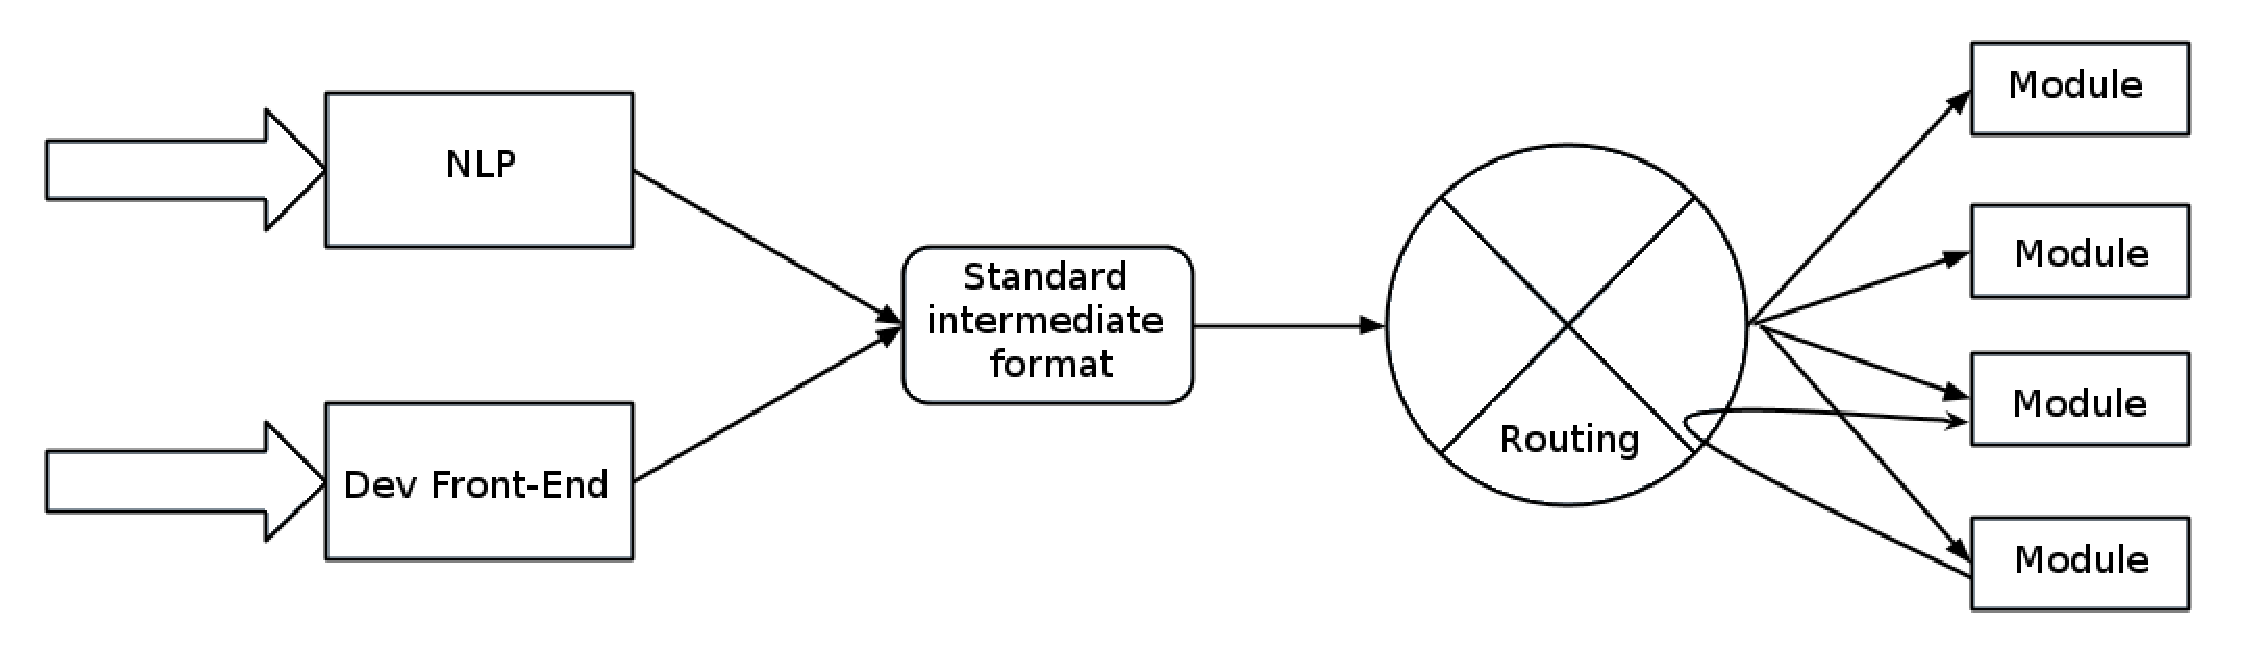
\includegraphics[scale=0.40]{images/Structure-PPP-en.eps}
    \caption{Global structure}
\end{figure}

The software is divided in several components which interact via the HTTP protocol.

The user interface consist of several front-ends. The most natural is
a web page, but we can also think about a Android application
or a Firefox OS web app. Via this interface, we can submit a query.

The query is transformed into a standard form. This form has to be understandable 
for a computer and describe the question. This work is done in two ways. There is 
a classical natural language processing module and a machine learning-based module. 
This kind of transformation is very difficult. To avoid having to go through this 
step, we can develop another front-end for developers which allow to input a question
 directly in normal form.

The standard form is sent into the core. The core's job is routing. It has to send 
the request in each module to obtain the answers. Sometime, a module can request 
an answer of another module, for example in the question \emph{What is two times the 
population of Argentina?} which needs a geographic data and a mathematical
 operation. Such a question needs the successive work of two modules.

To overcome the constraints of language, the core makes some request to the Wikidata
 module to translate each word of the standard form into the associated Wikidata 
 code.

Once a response is generated, it is sent to the interface to be displayed.

A specific module is needed for each database or kind of computation (mathematical, 
predictive machine learning\ldots).

\section{Technological innovations}

We would like to build one of the first open source question answering system. 
Our goal is to discover the theory of natural language processing, and apply our 
knowledge to design our tool. We intend to put together some existing libraries 
(e.g. natural language parsers) and our own implementations of algorithms. In 
particular, we hope we will be able to implement a neuronal network in order to 
perform machine learning. For example, we are going to explore deep learning
technologies for the natural language processing problem.

One of our most important goal is to provide the first full-modular question 
answering system. We do not pretend to build in 3 months a better tool than 
WolframAlpha for example, but we hope to make available an efficient and 
attractive system that will motivate people to integrate their own module in the 
tool. Thus, we think that using the HTTP protocol for the communication between 
modules is an important part of our project, because it will allow a wide variety 
of programming languages to design modules.

Finally, our technical approach consists in quickly obtaining first results and 
a first working tool. Thus, we could use existing libraries in a first time. Then, 
we will improve it depending on our remaining time.

\section{Schedule}

We have planned a simple schedule in two periods.

For the mid-term, we plan to have a functional developer front-end, core, the 
Wikidata module (with the transformation in standard form with Wikidata codes), 
a first approach of the natural language parser and a base for machine learning. 
With this base, the software should be able to answer simple questions using the 
developer interface.

For the final term, we plan to have an enhanced natural language parser (especially 
for the machine learning-based one), a simple web front-end and a fully operational 
Wikidata module.

Depending on the remaining time, we can develop other modules, e.g. modules for 
OEIS, mathematics\ldots Our objective is not to provide a lot of modules, but a 
modular tool with at least one ``demo-module'' using Wikidata.

\section{Task partition}

We decide to form three working teams with mid-term and final evaluations goals. Some of them
may be split after the mid-term evaluation.

A first team, composed of Thomas and Valentin, has to develop the core and the front-ends.
This work should not be too long, especially for the front-ends part. For the mid-term
we plan to have a working core, a basic HTML frontend and a developer frontend that would
allow input directly questions in the standard form. For the final evaluation, if there is time,
we will improve the HTML frontend and maybe build an Android application.

The second team will be charged with designing the first module, based on Wikidata. It is
composed of Thomas, Valentin and Tom. Thomas's knowledge on Wikidata will be essential
to make the work easier. The main goal is to have a module able to answer to simple questions
like \textit{When was Gandhi born?} for the mid-term. This team could eventually be
split after in a team for enhanced Wikidata module and another for making new modules.

The natural languages parsers (using eventually machine learning and neuronal networks) 
will be done by the last team composed of Yassine, Quentin, Raphaël and Marc. 
Since we cannot predict the difficulty of this task, we do not currently know if 
some members of this team will design other modules.
The goal for the mid-term is to have a first natural languages parser using intensively
existing libraries and a bibliographical study in order to understand how natural 
language parsers are designed, and then choose our own approach. We hope to be able 
to have an implemented machine learning algorithm based on neuronal networks for 
the final evaluation.

\section{Organization}

There will be several workpackages, and some manager associated to each one.
The role of these managers is to ensure the good progress of their workpackage.

\begin{tabular}{ll}
  Global organization & Marc\\
  System administration & Valentin\\
  Software architecture & Thomas\\
  Communication & Tom\\
  Bibliography & Yassine\\
  Router & Valentin\\
  Web user interface & Thomas\\
  Natural Languages Processing & Raphaël\\
  Machine Learning & Quentin\\
  Wikidata module & Thomas\\
  Add-ons & Marc\\
\end{tabular}

\begin{comment}
\begin{itemize}
    \item[Marc] is the project lead, whose task is also to make sure that the project is on the good way
    \item[Valentin] will do system administration (git repository infrastructure, continuous integration
    services, management of the demo server, \dots).
    \item[Thomas] is the software architect, whose task is to design the modular conception and to
    ensure that components fit well together.
\end{itemize}
\end{comment}

\section{Budget}
As demo servers will be provided by Wikimedia, we do not need any particular budget.

\section{Test protocol}

Evaluating a question answering system is quite a subjective task. Actually, we do not plan to have a full exhaustive test protocol. We will probably evaluate manually the relevance of our tool on some questions. Depending on its performances, we could also use existing benchmarks provided by question answering challenges (e.g. TREC challenge).

\end{document}
